\section{Numerical Experiments and Results}
\label{sec:results}

In this section we discuss various numerical experiments and results
concerning different variants of the preconditioner and comparisons of
solvers and boundary extrapolation methods.  Unless otherwise stated the
measurements are done on a tube embedded in a rectangular equidistant
$256\times256\times256$ grid.  This is a common problem size in beam
dynamics simulations.

Throughout this section we will report the timings of portions of the
code as listed in Table~\ref{tbl:timings_description}.
\begin{table}[ht]
  \begin{center}
    \begin{tabular}{ll}
      \hline
      name & description \\
      \hline
      construction & time for constructing the ML hierarchy \\
      application  & time for applying the ML preconditioner \\
      total ML     & total time used by ML ($=$ construction $+$ application) \\
      solution     & time needed by iterative solver \\
      \hline
    \end{tabular}
    \caption{Description of various timings used}
    \label{tbl:timings_description}
  \end{center}
\end{table}

\subsection{Comparison of Extrapolation Schemes}

For validation and comparison purposes we applied our solver to a
problem with a known analytical solution.  We solved the Poisson problem
with homogeneous Dirichlet boundary conditions ($\phi = 0$) on a
cylinderical domain $\Omega = \{ |r|<\frac{1}{2} \} \times
(-\frac{1}{2},\frac{1}{2})$.  The axisymmetric charge density
\begin{equation*}
  \rho = -\left( \pi^2 r^2 - \frac{\pi^2}{4} - 4 \right)
  \sin(\pi(z-0.5))
\end{equation*}
gives rise to the potential distribution
%
\begin{equation*}
  \phi(r, \theta, z) = \left( \frac{1}{4}-r^2 \right) \sin(\pi(z-0.5)).
\end{equation*}
The charge density in our test problem is smoother than in real
problems.  Nevertheless, it is very small close to the boundary.  This
reflects the situation in particle accelerators where most particles are
close to the axis of rotation and, thus, charge densities are very small
close to the boundary. 
% For this reason, we do not expect the boundary treatment to be a
% crucial issue of our simulations.

To measure the error on the grid $\Omega_h$ with mesh spacing $h$ in the
discrete norms
%
\begin{gather*}
  \Vert e_h \Vert_2 = \Vert \hat{\phi}_h - \phi
  \Vert_2 =  \sqrt{h^3 \sum_{i \in 
      \Omega_h} \vert (\hat{\phi}_{i,h}-\phi_i)\vert^2}, \\
  \Vert e_h \Vert_\infty = \Vert \hat{\phi}_h - \phi
  \Vert_\infty =  \max_{i \in \Omega_h} 
  \vert \hat{\phi}_{i,h} - \phi_i \vert,
\end{gather*}
where $\hat{\phi}_h$ is the approximation of the solution $\phi$ on
$\Omega_h$ and $e_h$ denotes the corresponding error.
%
The convergence rate $r$ is defined by
%
\begin{equation*}
  r = \log_2 \left( \frac{\vert\vert e_{2h} \vert\vert}{\vert\vert e_h
      \vert\vert} \right).
\end{equation*}
%
\begin{table*}[htb]
  \begin{center}
    \begin{tabular}{llllll}
      \hline
      $h$ & $\vert\vert e_h \vert\vert_2$ & $r$ & $\vert\vert e_h
      \vert\vert_\infty$ & $r$ & $\vert\vert e_h \vert\vert_\infty /
      \vert\vert \phi \vert\vert_\infty$ \\ [0.2ex] \hline 
      \vphantom{\rule{0pt}{2.7ex}}
      $1/64$  & $2.162 \times 10^{-3}$ & & $7.647 \times 10^{-3}$ & &
      $3.061 \times 10^{-2}$ \\ 
      $1/128$ & $1.240 \times 10^{-3}$ & 0.80 & $4.153 \times 10^{-3}$ &
      0.88 & $1.662 \times 10^{-2}$ \\ [0.2ex]
      \hline
    \end{tabular}
    \caption{Solution error for constant extrapolation, $d=3$}
    \label{tbl:rel_error_const}
  \end{center}

  \begin{center}
    \begin{tabular}{llllll}
      \hline
      $h$ & $\vert\vert e_h \vert\vert_2$ & $r$ & $\vert\vert e_h
      \vert\vert_\infty$ & $r$ & $\vert\vert e_h \vert\vert_\infty /
      \vert\vert \phi \vert\vert_\infty$\\ [0.2ex]
      \hline 
      \vphantom{\rule{0pt}{2.7ex}}
      $1/64$  & $2.460 \times 10^{-5}$ & & $6.020 \times 10^{-5}$ & &
      $2.410 \times 10^{-4}$ \\
      $1/128$ & $6.226 \times 10^{-6}$ & 1.98 & $1.437 \times 10^{-5}$ &
      2.07 & $5.751 \times 10^{-5}$ \\ [0.2ex]
      \hline
    \end{tabular}
    \caption{Solution error for linear extrapolation, $d=3$}
    \label{tbl:rel_error_lin}
  \end{center}

  \begin{center}
    \begin{tabular}{llllll}
      \hline
      $h$ & $\vert\vert e_h \vert\vert_2$ & $r$ & $\vert\vert e_h
      \vert\vert_\infty$ & $r$ & $\vert\vert e_h \vert\vert_\infty /
      \vert\vert \phi \vert\vert_\infty$\\ [0.2ex]
      \hline 
      \vphantom{\rule{0pt}{2.7ex}}
      $1/64$  & $5.581 \times 10^{-6}$ & & $1.689 \times 10^{-5}$ & &
      $6.761 \times 10^{-5}$ \\ 
      $1/128$ & $1.384 \times 10^{-7}$ & 2.01 & $4.550 \times 10^{-6}$ &
      1.89 & $1.820 \times 10^{-5}$ \\ [0.2ex]
      \hline
    \end{tabular}
    \caption{Solution error for quadratic extrapolation, $d=3$}
    \label{tbl:rel_error_quad}
  \end{center}
\end{table*}

We solved the Poisson equation with the boundary extrapolation methods
introduced earlier.  The errors are listed in
Tables~\ref{tbl:rel_error_const}--\ref{tbl:rel_error_quad}.  The numbers
confirm the expected convergence rates.  The results obtained with the
linear extrapolation scheme are more accurate than constant
extrapolation by two orders of magnitude.  Quadratic extrapolation is
again more accurate than linear extrapolation, but for both norms by
only a factor~3 to~5.  It evidently does not make sense to use constant
extrapolation as the cost of solving with linear boundary extrapolation
is equal.  In contrast, the quadratic boundary treatment entails the
drawback that discretization matrices become nonsymmetric positive
definite.  However, in the particular setting of this test problem as
well as in others we have investigated (e.g.\ in real particle
simulations) the system matrices were just mildly nonsymmetric such that
PCG could be applied savely and without performance loss.


% under consideration has not been chosen arbitrary.
% For instance the smoothness characteristic concurs with charge densities
% appearing in our particle accelerator simulations. One small difference
% concerns the behaviour at the boundary.  In simulations we usually have
% particles closer to the axis of rotation in contrast to this charge
% density with non-zeros values at the boundary.  This will mainly be
% responsible for accuracy discrepancies between linear and quadratic
% extrapolation schemes.

\subsection{ML variations}\label{sec:ml_var}

Multilevel preconditioners are highly sophisticated preconditioners.
Not surprisingly, their construction is very time consuming.  To build
an SA-AMG preconditioner (1) the ``grid'' hierarchy (including
aggregation and construction of tentative prolongator), (2) the final
grid transfer operators (smoothing the prolongators), and (3) the coarse
grid solver have to be set up.

In the following subsections we investigate various variants of the
preconditioner or more precisely variants of the construction of the
preconditioner when solving a sequence of related Poisson problems.
%The goal is to decrease the time-to-solution.

The default variant builds a new preconditioner in every time step.  In
the sequel we will investigate how costly this is.  Other variants reuse
portions of previous preconditioners.

We compare with the FFT-based Poisson solver~\cite{hoea:88} that
\textsc{OPAL} provides for open-space boundary conditions.  The current
version (1.1.5) uses a variant of the FFTPACK library to compute
FFT's~\cite{FFTPACK, Swar:82}.

\subsubsection*{Reusing the aggregation hierarchy}

Since the geometry often changes only slowly in time, the
\emph{topology} of the computational grid does not or only rarely alter.
Therefore, it makes sense to reuse the aggregation hierarchy and in
particular the tentative prolongators for some or all iterations.  Only
smoothed prolongators and other components of the hierarchy, like
smoothers and coarse solver, are recomputed~\cite[p.16]{gsht:06}.
%%
%%The most straightforward improvement presents itself with the insight
%%that the geometries usually vary slowly or not at all in time.  In this
%%case it makes no sense to discard the information about the aggregation
%%hierarchy computed in the last time-step.  
This leads to a preconditioner variation in which the aggregation
hierarchy is kept as long as possible.  The numbers in
Table~\ref{tbl:timings_reuse_hierarchy} show that this minor change in
the set up phase reduces construction times by approximately 30\%.

\begin{table}[ht]
  \begin{center}
    \begin{tabular}{ccc}
      \hline
      \rule{15mm}{0mm} & \rule{30mm}{0mm} & \rule{30mm}{0mm} \\[-4mm]
      cores & average of 10 & one \\
      &time steps (s) &  time step (s) \\
      \hline
      16  & 6.98 & 10.3 \\
      32  & 4.36 &  6.44 \\
      64  & 2.38 &  3.48 \\
      128 & 1.34 &  1.91 \\ 
      256 & 0.735 &  1.04 \\
      512 & 0.518 &  0.745 \\
      \hline
    \end{tabular}
    \caption{Construction times in seconds for 10 time-steps reusing
      hierarchy vs 1 time-step building hierarchy}
    \label{tbl:timings_reuse_hierarchy}
  \end{center}
\end{table}

Reusing the aggregation hierarchy is a feature provided by ML.  It is
intended for use in nonlinear systems solving.  In our simulations it
reduced the time per AMG solve in a simulation run by approximately
25\%, see Table~\ref{tbl:timings_variations_overview}.

\subsubsection*{Reusing the preconditioner}

We can be more aggressive by reusing the preconditioner of the first
iteration throughout a whole simulation.  Although the iteration count
increased, the time-to-solution reduced considerably.  To counteract an
excessive increase of the iteration steps we can recompute the
preconditioner once the number of iterations exceeds a certain
threshold.  (This was not necessary in our experiments, though.)

Applying this approach to a cylinder-shaped beam pipe, a single
preconditioner could be used throughout the entire simulation without
any severe impact on the number of iteration steps.

\begin{figure}[ht]
  \begin{minipage}[b]{0.5\textwidth}
    \centering
    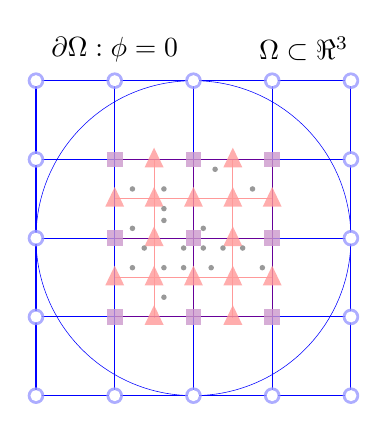
\begin{tikzpicture}[domain=-0.2:4.2,scale=1.0]
    %MG grid
    \draw[thin,color=blue,step=10mm] (0.0,0.0) grid (4,4);
    %\draw[very thin,color=gray,step=2.5mm] (0.5,-0.2) grid (3.5,1.5);
    
    %labels
    \node at (3.4,4.4) {$\Omega \subset \Re^3$};
    \node at (1,4.4) {$\partial \Omega: \phi = 0$};

    %additional grid lines MG
    %\draw[thin,color=blue] (0.5,0.0) to (0.5,4);
    %\draw[thin,color=blue] (1.5,0.0) to (1.5,4);
    %\draw[thin,color=blue] (2.5,0.0) to (2.5,4);
    %\draw[thin,color=blue] (3.5,0.0) to (3.5,4);
    
    \draw[very thin,color=blue] (2.0,2.0) circle (2);
    
    %FFT grid
    \draw[thin,color=red,step=5mm,opacity=0.4] (1.0,0.99) grid (3,3);

    %MG meshpoints
    \foreach \i in {0, 1.0, ..., 4}
    {
        \fill[blue!40,opacity=0.8] (\i,0.0) circle (3pt);
        \fill[white,opacity=1.0] (\i,0.0) circle (2pt);
    }
    \foreach \i in {0, 1.0, ..., 4}
    {
        \fill[blue!40,opacity=0.8] (\i,4.0) circle (3pt);
        \fill[white,opacity=1.0] (\i,4.0) circle (2pt);
    }
    \foreach \i in {1, ..., 3}
    {
        \fill[blue!40,opacity=0.8] (0.0,\i) circle (3pt);
        \fill[white,opacity=1.0] (0.0,\i) circle (2pt);
    }
    \foreach \i in {1, ..., 3}
    {
        \fill[blue!40,opacity=0.8] (4.0,\i) circle (3pt);
        \fill[white,opacity=1.0] (4.0,\i) circle (2pt);
    }
    
    %FFT meshpoints
    \foreach \i in {1, 1.5, ..., 3}
    {
        \fill[red!40,opacity=0.8] (\i-0.12,1.5-0.1) -- (\i,1.5+0.15) -- (\i+0.12,1.5-0.1);
    }
    \foreach \i in {1, 1.5, ..., 3}
    {
        \fill[red!40,opacity=0.8] (\i-0.12,2.5-0.1) -- (\i,2.5+0.15) -- (\i+0.12,2.5-0.1);
    }
    \foreach \j in {1.0, ..., 3.0}
    {
        \foreach \i in {1.5, ..., 2.5}
        {
            \fill[red!40,opacity=0.8] (\i-0.12,\j-0.1) -- (\i,\j+0.15) -- (\i+0.12,\j-0.1);
        }
    }
   
    %SHARED meshpoints
    \foreach \j in {1, ..., 3}
    {
        \foreach \i in {1, ..., 3}
        {
            \fill[violet!40,opacity=0.8] (\i-0.1,\j-0.1) rectangle (\i+0.1,\j+0.1);
        }
    }


    %particles
    \fill[black!40] (2.225,1.625) circle (1pt);
    \fill[black!40] (2.750,2.625) circle (1pt);
    \fill[black!40] (1.625,1.25) circle (1pt);
    
    \fill[black!40] (2.275,2.875) circle (1pt);

    \fill[black!40] (1.625,2.625) circle (1pt);
    
    \fill[black!40] (1.375,1.875) circle (1pt);

    \fill[black!40] (1.225,2.625) circle (1pt);
    \fill[black!40] (1.225,2.125) circle (1pt);
    \fill[black!40] (1.225,1.625) circle (1pt);
    
    \fill[black!40] (1.625,2.375) circle (1pt);
    \fill[black!40] (1.625,1.625) circle (1pt);
    \fill[black!40] (1.625,2.225) circle (1pt);

    \fill[black!40] (1.875,1.875) circle (1pt);
    \fill[black!40] (1.875,1.625) circle (1pt);
    
    \fill[black!40] (2.125,1.875) circle (1pt);
    \fill[black!40] (2.125,2.125) circle (1pt);

    \fill[black!40] (2.375,1.875) circle (1pt);

    \fill[black!40] (2.625,1.875) circle (1pt);
    
    \fill[black!40] (2.875,1.625) circle (1pt);

\end{tikzpicture}


    (a)
  \end{minipage}
  %\hspace{0.2cm}
  \begin{minipage}[b]{0.5\textwidth}
    \centering
    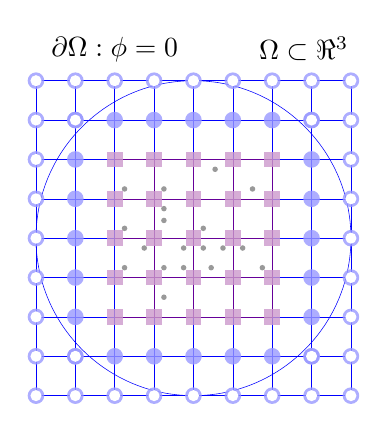
\begin{tikzpicture}[domain=-0.2:4.2,scale=1.0]
    \draw[very thin,color=blue,step=5mm] (0.0,0.0) grid (4,4);
    \draw[very thin,color=red,step=5mm,opacity=0.4] (1.0,0.99) grid (3,3);
    %\draw[very thin,color=gray,step=2.5mm] (0.5,-0.2) grid (3.5,1.5);
    
    %\filldraw[fill=gray!20,fill opacity=0.8](2,2)--(2,3)--(3,3)--(3,2)--cycle;

    %curved boundart
    %\draw (-0.2,3.55) to[out=20,in=180] node [sloped,below] {} (4.2,3.8);
    %\draw (-0.2,3.3) to[out=30,in=180] node [sloped,below] {$\Omega$} (4.2,3.8);
    
    %\coordinate [label=above:\C] (C) at (intersection of B and 1,0--1,1);
    %\fill[black,opacity=.5] C circle (2pt);
    
    \draw[very thin,color=blue] (2.0,2.0) circle (2);
  
    %labels
    \node at (3.4,4.4) {$\Omega \subset \Re^3$};
    \node at (1,4.4) {$\partial \Omega: \phi = 0$};

    \foreach \i in {0, 0.5, ..., 4}
    {
        \fill[blue!40,opacity=0.8] (\i,0.0) circle (3pt);
        \fill[white,opacity=1.0] (\i,0.0) circle (2pt);
    }
    \foreach \i in {0.5, 1.0, ..., 3.5}
    {
        \fill[blue!40,opacity=0.8] (\i,0.5) circle (3pt);
    }

    \foreach \i in {0.5, 1.0, ..., 3.5}
    {
        \fill[blue!40,opacity=0.8] (\i,3.5) circle (3pt);
    }
    \foreach \i in {0, 0.5, ..., 4}
    {
        \fill[blue!40,opacity=0.8] (\i,4.0) circle (3pt);
        \fill[white,opacity=1.0] (\i,4.0) circle (2pt);
    }
    
    \foreach \i in {1, 1.5, ..., 3}
    {
        \fill[blue!40,opacity=0.8] (0.0,\i) circle (3pt);
        \fill[white,opacity=1.0] (0.0,\i) circle (2pt);
    }
    \foreach \i in {1, 1.5, ..., 3}
    {
        \fill[blue!40,opacity=0.8] (0.5,\i) circle (3pt);
    }
    \foreach \i in {1, 1.5, ..., 3}
    {
        \fill[blue!40,opacity=0.8] (3.5,\i) circle (3pt);
    }
    \foreach \i in {1, 1.5, ..., 3}
    {
        \fill[blue!40,opacity=0.8] (4.0,\i) circle (3pt);
        \fill[white,opacity=1.0] (4.0,\i) circle (2pt);
    }
    \fill[blue!40,opacity=0.8] (3.5,3.5) circle (3pt);
    \fill[white,opacity=1.0] (3.5,3.5) circle (2pt);
    \fill[blue!40,opacity=0.8] (4.0,3.5) circle (3pt);
    \fill[white,opacity=1.0] (4.0,3.5) circle (2pt);
    
    \fill[blue!40,opacity=0.8] (0.5,3.5) circle (3pt);
    \fill[white,opacity=1.0] (0.5,3.5) circle (2pt);
    \fill[blue!40,opacity=0.8] (0.0,3.5) circle (3pt);
    \fill[white,opacity=1.0] (0.0,3.5) circle (2pt);
    
    \fill[blue!40,opacity=0.8] (3.5,0.5) circle (3pt);
    \fill[white,opacity=1.0] (3.5,0.5) circle (2pt);
    \fill[blue!40,opacity=0.8] (4.0,0.5) circle (3pt);
    \fill[white,opacity=1.0] (4.0,0.5) circle (2pt);
    
    \fill[blue!40,opacity=0.8] (0.5,0.5) circle (3pt);
    \fill[white,opacity=1.0] (0.5,0.5) circle (2pt);
    \fill[blue!40,opacity=0.8] (0.0,0.5) circle (3pt);
    \fill[white,opacity=1.0] (0.0,0.5) circle (2pt);
        
   
    \foreach \j in {1, 1.5, ..., 3}
    {
        \foreach \i in {1, 1.5, ..., 3}
        {
            \fill[violet!40,opacity=0.8] (\i-0.1,\j-0.1) rectangle (\i+0.1,\j+0.1);
        }
    }

    %\fill[violet!40,opacity=0.8] (-0.1,0.9) rectangle (0.1,1.1);
    %\fill[violet!40,opacity=0.8] (0.4,0.9) rectangle (0.6,1.1);
    %\fill[violet!40,opacity=0.8] (0.9,0.9) rectangle (1.1,1.1);

    %particles
    \fill[black!40] (2.225,1.625) circle (1pt);
    \fill[black!40] (2.750,2.625) circle (1pt);
    \fill[black!40] (1.625,1.25) circle (1pt);
    
    \fill[black!40] (2.275,2.875) circle (1pt);

    \fill[black!40] (1.625,2.625) circle (1pt);
    
    \fill[black!40] (1.375,1.875) circle (1pt);

    \fill[black!40] (1.125,2.625) circle (1pt);
    \fill[black!40] (1.125,2.125) circle (1pt);
    \fill[black!40] (1.125,1.625) circle (1pt);
    
    \fill[black!40] (1.625,2.375) circle (1pt);
    \fill[black!40] (1.625,1.625) circle (1pt);
    \fill[black!40] (1.625,2.225) circle (1pt);

    \fill[black!40] (1.875,1.875) circle (1pt);
    \fill[black!40] (1.875,1.625) circle (1pt);
    
    \fill[black!40] (2.125,1.875) circle (1pt);
    \fill[black!40] (2.125,2.125) circle (1pt);

    \fill[black!40] (2.375,1.875) circle (1pt);

    \fill[black!40] (2.625,1.875) circle (1pt);
    
    \fill[black!40] (2.875,1.625) circle (1pt);

\end{tikzpicture}


    (b)
  \end{minipage} 
  \caption{Sketch of the test cases with equal number of mesh points
    (a), and equal mesh resolution (b), respectively.  Displayed are the
    shared (square), FFT only (triangle), and AMG only (circle) mesh
    points on a cross section of the grid plane.  Illustrative particles
    (gray) inside the FFT domain denote the charge density.}

  \label{fig:meshcmp}
\end{figure}

In the following we try to compare accuracy and performance of the
SA-AMG preconditioned conjugate gradient algorithm with a FFT-based
solver.  The principle difficulty in the comparison stems from the fact
that the CG-based and the FFT-based solvers use different
discretizations of the tube-shaped domain~$\Omega$.  Although both use
finite-difference discretizations, with SA-AMG the whole domain is
discretized while with FFT just a rectangular domain along the center
line of the cylinder is taken into account.  In some applications
({\color{red}???}) the rectangular domain is contained in $\Omega$.  In
our application the rectangular domain has a similar volume such that
the boundaries can be intertwined.  Therefore, we expect that the more
accurate boundary treatment in the iterative solver has a noticeable
positive effect on the solution.

So, we came up with two test cases as illustrated in
Figure~\ref{fig:meshcmp}.
\begin{itemize}
\item The first test case (a) displayed on the left corresponds to a
  situation where both methods have about the same number of unknowns.
  In the FFT-based approach only the close vicinity of the particle
  bunch is discretized.  In contrast, in the CG approach the grid
  extends to the whole domain, entailing a coarser grid than with the
  FFT-based approach.

\item The second test case (b) displayed on the right corresponds to a
  situation where both methods have the same mesh resolution in the
  vicinity of the particles.  This results in a higher number of mesh
  points for the PCG-AMG approach.
\end{itemize}
% The size of the domain in case of AMG is given by a radius and will be
% denoted by $r$.  On the other hand the size of the domain for the FFT
% method is determined by the size of the particle bunch.  Note that AMG
% domains are generally tubes in contrast to rectangular domains used by
% the FFT method.

The first test case consisted of a simulation of ??? within a
cylindrical tube of radius $r=0.003$\,m.  The FFT-based solver used a
grid with $256^2\cdot128=8388608$ nodes.  The iterative solver was run
with a grid consisting of ???  points.  The boundary conditions are
implemented by linear extrapolation.  3500~time steps were executed.  In
Table~\ref{tbl:timings_variations_overview} the average execution time
of one step are given.  The CG-AMG solver outperformed the FFT solver.
The improvement from the straightforward mode to the two cases reusing
either hierarchy or the entire preconditioner amounts to approximately
$20\%$ and $40\%$ respectively.
%%
\begin{table}[ht]
  \begin{center}
    \begin{tabular}{*{6}{c}}
      \hline
      solver & reusing & extrapolation & mesh points & solve [s] \\
      \hline 
      FFT & --- & --- & ??? & 25.4  \\
      AMG & --- & constant & ??? & 10.7  \\
      AMG & hierarchy & constant & ??? & 8.2  \\
      AMG & preconditioner & constant & ??? &6.7  \\
      \hline
    \end{tabular}
    \caption{Simulation timings of one solve averaged over $3500$
      time steps on a $256\times256\times128$
      grid} %% where $r=0.003$\,m}
    \label{tbl:timings_variations_overview}
  \end{center}
\end{table}

The second test case consisted of ??? with a cylindrical tube of radius
$r=0.001$\,m.  The FFT-based solver used a grid with
$128^2\cdot256=4'194'304$ nodes.  To obtained the same resolution with
the CG-AMG solver, 7'054'336 grid points were required.  They are
imbeded in a $166\times166\times256$ grid that coincides in the middle
of the region of simulation with the $128\times128\times256$ grid for
the FFT-based solver.  Again, the boundary conditions are implemented by
linear extrapolation.

\begin{table}[ht]
  \begin{center}
    \begin{tabular}{cccccc}
    \hline
        solver & reusing & mesh size & mesh points & solve [s] & $\infty$ [s] \\
        \hline
        FFT & --- & $128\times128\times256$ & 4194304 & 16.9 & --- \\
        AMG & --- & $166\times166\times256$ & 7054336 & 84.28 & 84.28 \\
        AMG & hierarchy & $166\times166\times256$ & 7054336 & 75.42 & 66.56 \\
        AMG & preconditioner & $166\times166\times256$ & 7054336 & 69.11 & 53.94 \\
        \hline
  \end{tabular}
  \caption{Simulation timings of one solve averaged over two time steps
    with $r=0.001$\,m.  Equal mesh spacings for FFT and AMG.}
  \label{tbl:timings_variations_overview_fixmeshspacings} \end{center}
\end{table}
%%


To achieve the same resolution (mesh spacings) at particles as in the
FFT simulations we need $2860032$ additional mesh points for AMG.

The results in
Table~\ref{tbl:timings_variations_overview_fixmeshspacings} indicate
that the additional mesh points considerably hurt the performance of the
AMG solver.  Why so much???  Iteration count???

To examine the influence (on what) of the resolution in this particular
case we conducted additional simulation runs employing the same number
of mesh points for AMG.  (Equal grids should give equal results!!??)
The simulation for the same number of mesh points yields in this
particular case exactly the same results compared to simulation
maintaining the same resolution at particles.

Again we measure approximately a 20\% (respectively 40\%) reduction of
time when reusing hierarchy and preconditioner.

%Since the two methods differ in many ways it is very delicate to conduct a
%satisfying comparison.

\subsubsection*{Coarse level solver}

Another decisive portion of the AMG preconditioner is the coarse level
solver.  We applied either a direct solver (KLU) or used a couple of
steps of Gauss-Seidel iteration.  The timings in
Table~\ref{tab:gs_vs_klu} indicate that for our problems ML setup time
and scalability are not affected significantly by the two coarse level
solvers.  However, the construction of the preconditioner is cheaper
with the iterative coarse level solver.  

As stated by Tuminaro \& Tong~\cite{tuto:00} the number of iterations
done by the iterative coarse level solver is crucial for the the
performance of the preconditioner.  Too many iteration steps slow down
the preconditioner without a corresponding increase of its quality.  Too
few iteration steps with the coarse level solver degrade the quality of
the overall preconditioner and lead to an increased number of steps of
the global system solver.  We tuned the iterative coarse level solver
such that the overall quality of the preconditioner was about the same
as with the direct coarse level solver.  It turned out that 3~iteration
steps were enough.

%The relaxation of the approximation quality entails an increase of the steps of
%the overall PCG iteration.

\begin{table}[ht]
  \begin{center}
    \begin{tabular}{cccccccc}
      \hline
      \multirow{2}{*}{cores} & \multicolumn{3}{c}{KLU [s]} & &
      \multicolumn{3}{c}{Gauss-Seidel [s]} \\
      \cline{2-4} \cline{6-8}
      &  construction & all applications & total ML & & construction & all
      applications & total ML\\
      \hline
      16  & 10.44 & 13.58 & 24.02 & & 10.27 & 13.54 & 23.81 \\
      32  & 6.69 & 8.48 & 15.18 & & 6.44 & 8.41 & 14.85 \\
      64  & 3.91 & 4.31 & 8.21 & & 3.48 & 4.49 & 7.97 \\
      128 & 1.93 & 2.21 & 4.23 & & 1.91 & 2.28 & 4.18 \\
      256 & 1.14 & 1.39 & 2.53 & & 1.04 & 1.36 & 2.40 \\
      512 & 1.07 & 0.96 & 2.03 & & 0.74 & 0.92 & 1.66 \\
      \hline
    \end{tabular}
    \caption{KLU vs.\ Gauss-Seidel (1) as coarse level
    solver}\label{tab:gs_vs_klu} \end{center}
%  \begin{center}
%    \begin{tabular}{cccc}
%      \hline
%      cores &  construction [s] & all applications [s] & total ML [s] \\
%%           &  (s) & (s) & (s) \\
%      \hline
%      16  & 10.27 & 13.54 & 23.81 \\
%      32  & 6.44 & 8.41 & 14.85 \\
%      64  & 3.48 & 4.49 & 7.97 \\
%      128 & 1.91 & 2.28 & 4.18 \\ 
%      256 & 1.04 & 1.36 & 2.40 \\
%      512 & 0.74 & 0.92 & 1.66 \\
%      \hline
%    \end{tabular}
%    \caption{3 iterative solver steps at coarsest level}
%    \label{tab:v_smooth}
%  \end{center}
\end{table}

\subsubsection*{Coarse level size}

We also tested the performance of the solver for varying sizes of the
coarsest level.  ML seems to perform best when the coarsest grid size is
around 1000.  With a limit of 1000, the coarsest grid sizes ranged from
128 to 849 when running a tube embedded in a $256 \times 256 \times 256$
grid on 16 to 512 cores.

At the same time we tried to set the size of the coarsest level
proportional to the total available number of cores in order to get a
sufficient large coarse level size.  It turned out to be very difficult
to set a coarse level size with heuristics like this.  The factorization
time increased to up to 2\,s in contrast to $0.25$\,s for the case where
the coarsest level size is limited by~1000.


\subsection{Speedup and efficiency}

The efficiency of the AMG solver using linear boundary extrapolation is
shown in Figure~\ref{fig:speedup}.  On the left of this figure, the
results listed in Tab.~\ref{tbl:timings_solver} for a $256^3$ grid are
plotted.  We observe an efficiency of approximately 62\% for 256 cores
relative to the timing on 16~processors, the minimal number of
processors to solve the problem.  The efficiency dropped just below 50\%
for 512 cores.  The parallel efficiency is affected most by the poor
scalability of the construction phase of ML.  After studying various ML
timings we could not identify a specific reason that causes this loss in
efficiency for the construction phase other than the assumption that the
problem is too small with respect to the number of cores.

\begin{figure}[htb] 
  \begin{center}
    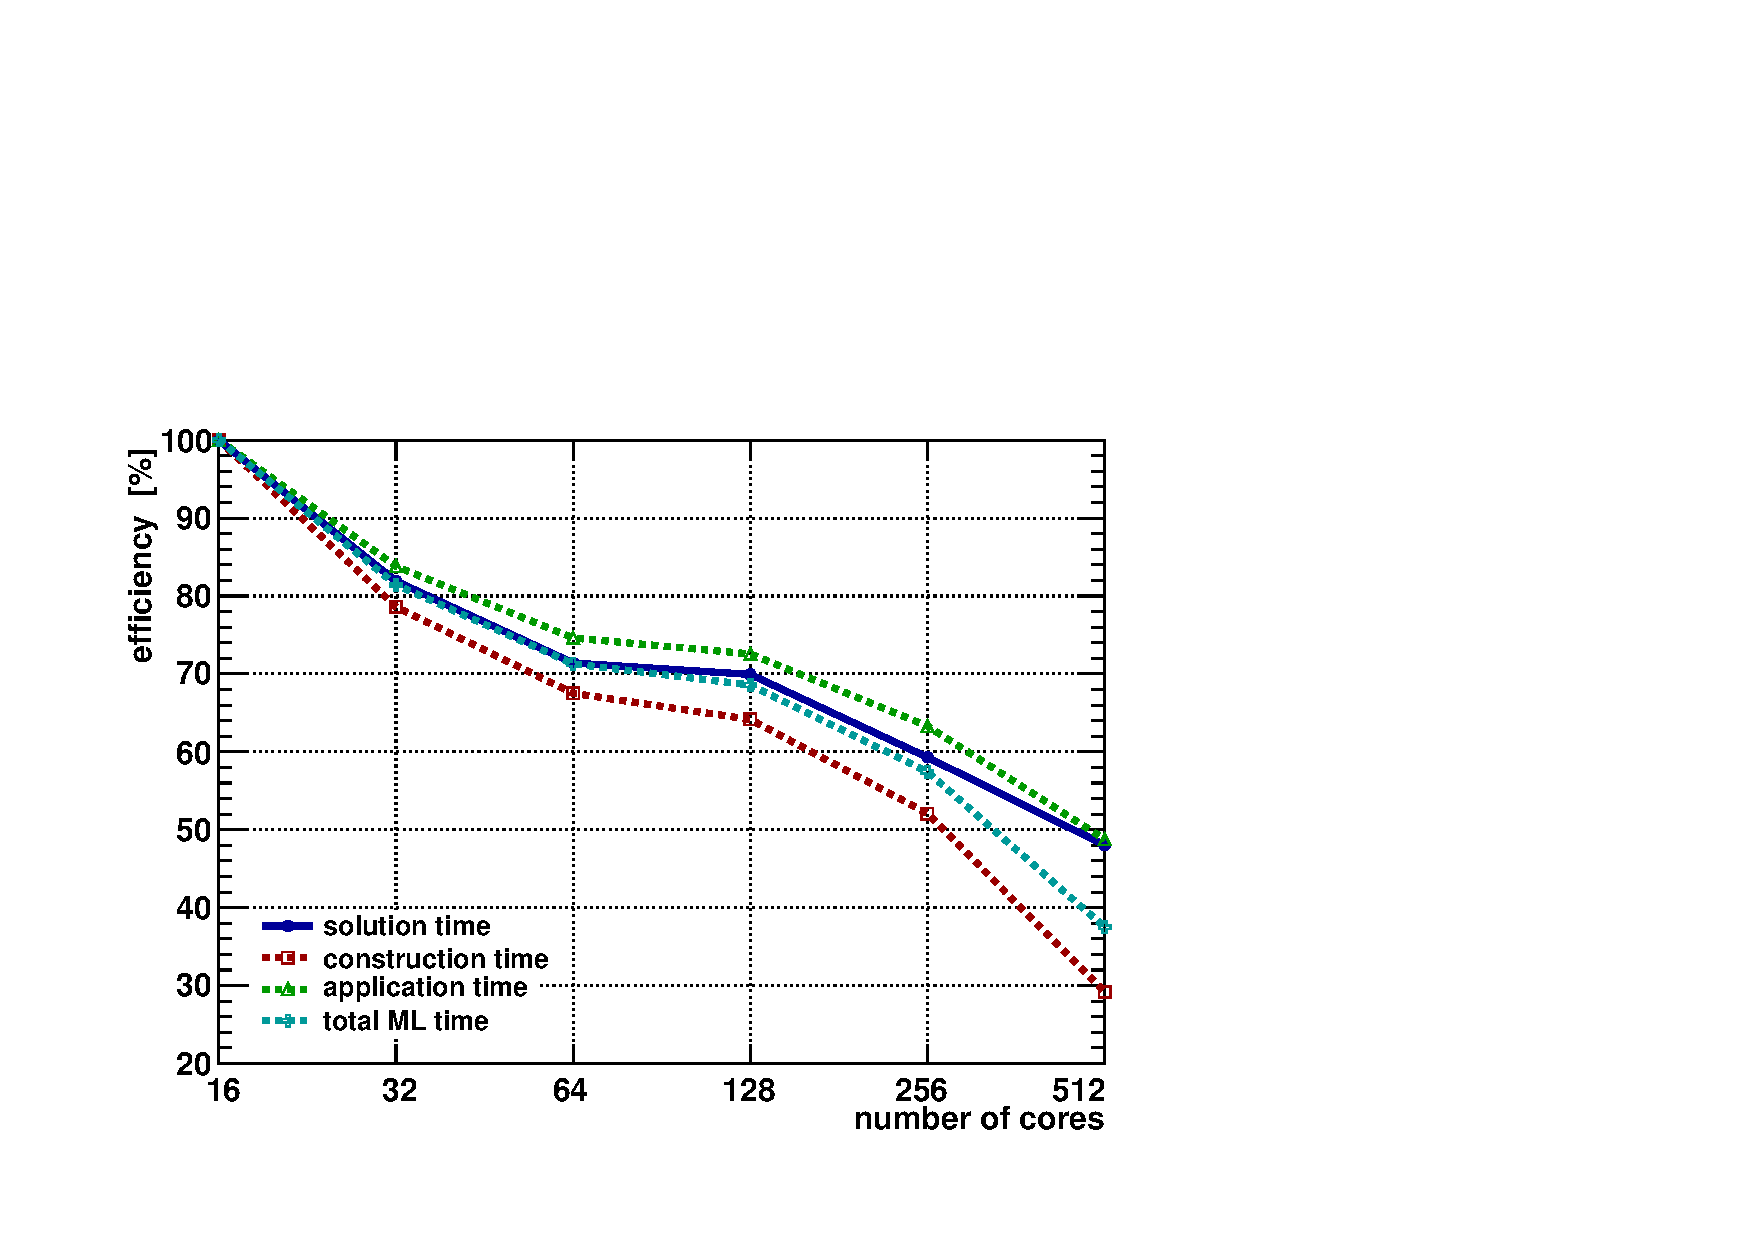
\includegraphics[width=0.45\textwidth]{figures/eff_256.pdf}
    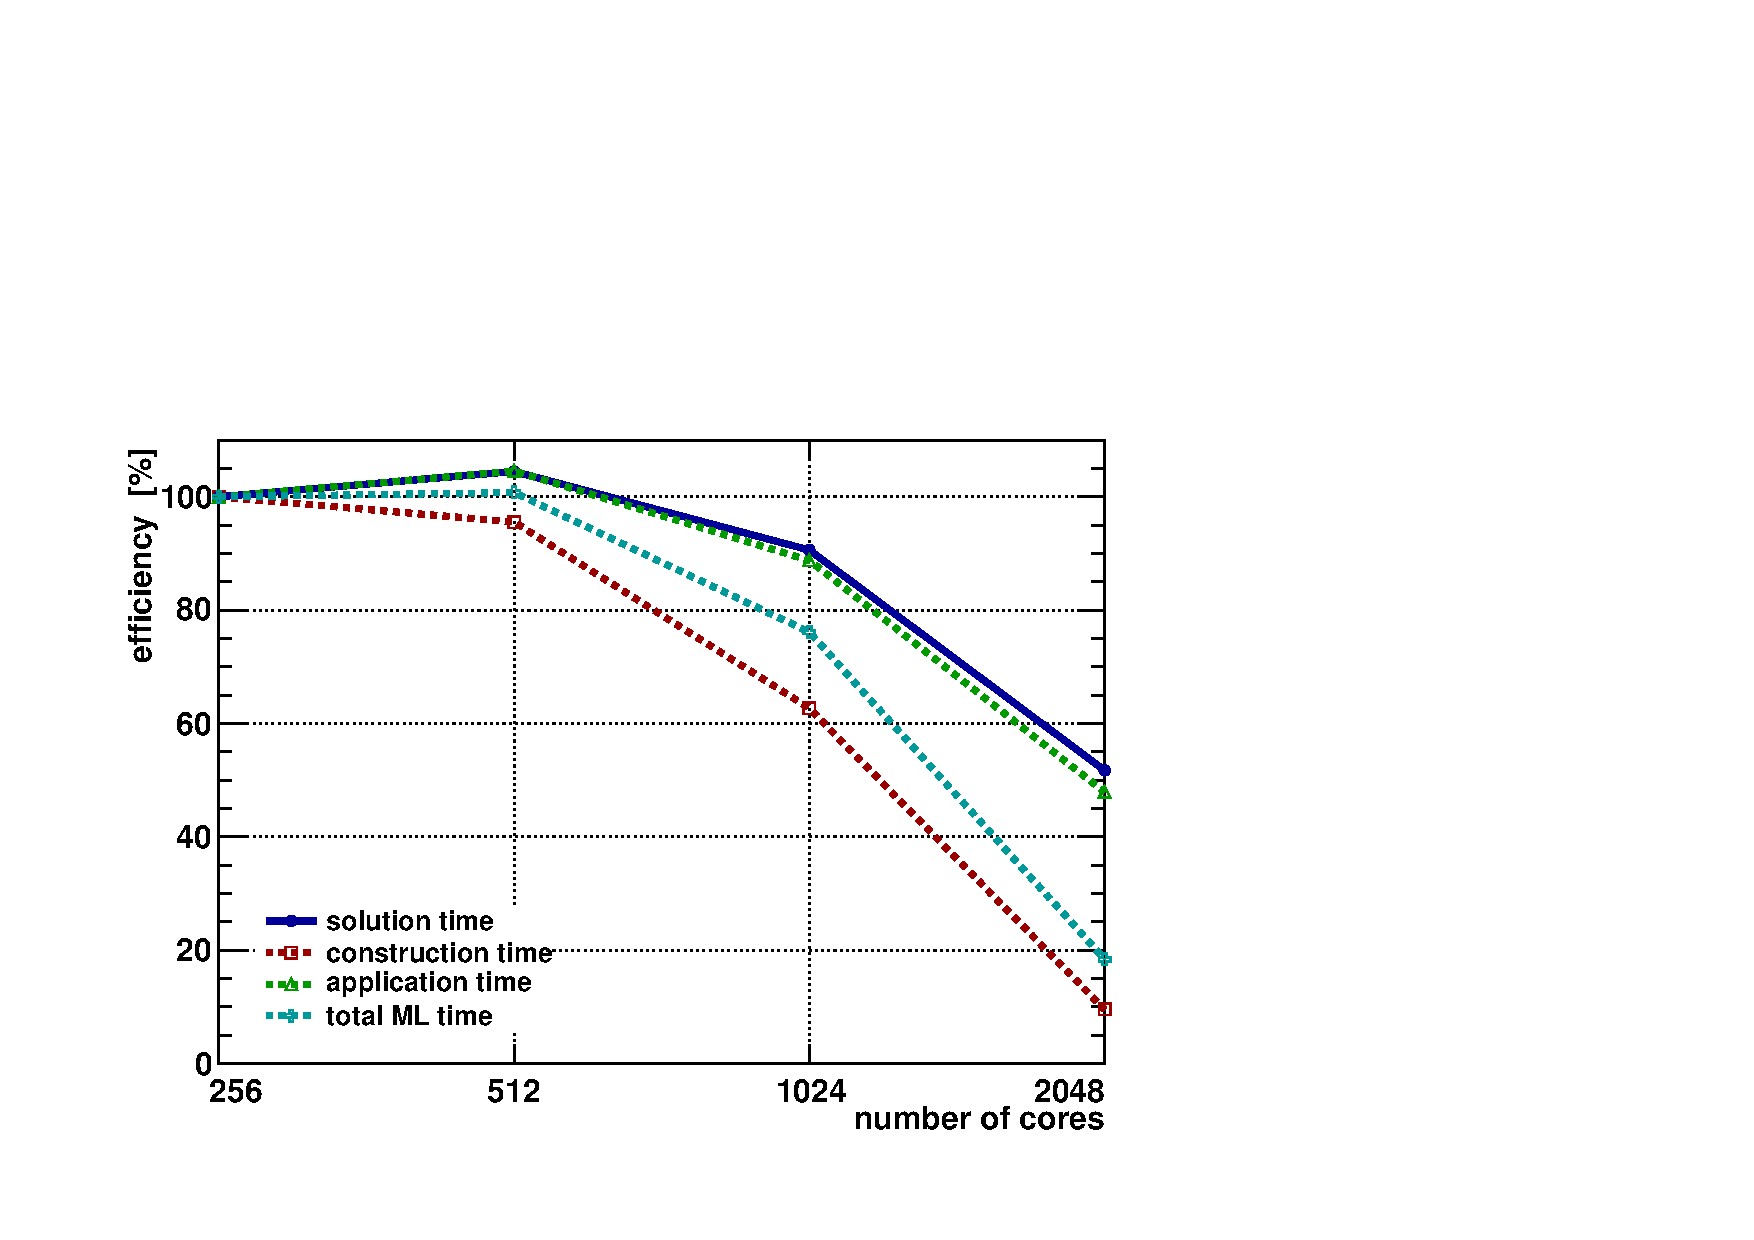
\includegraphics[width=0.45\textwidth]{figures/eff_512.pdf}
    \caption{Efficiency for AMG on a tube embedded in a
      $256\times256\times256$ grid (left) and in a
      $512\times512\times512$ grid (right) with constant extrapolation
      at the boundary.}
    \label{fig:speedup}
  \end{center} 
\end{figure}

\begin{table}[htb]
  \begin{center}
    \begin{tabular}{ccccc}
      \hline
      cores & solution [s] & construction [s] & application [s] & total ML [s] \\
%            & (s) & (s) & (s) & (s) \\
      \hline
      16  & 10.91 &  7.75 &  9.52 & 17.28 \\
      32  &  6.66 &  4.93 &  5.68 & 10.61 \\
      64  &  3.82 &  2.87 &  3.19 &  6.06 \\
      128 &  1.95 &  1.51 &  1.64 &  3.15 \\
      256 &  1.15 &  0.93 &  0.94 &  1.88 \\
      512 &  0.71 &  0.83 &  0.61 &  1.44 \\
      \hline
    \end{tabular}
    \caption{Timings for AMG on a tube embedded in a $256\times256\times256$
      grid with linear extrapolation at the boundary}
    \label{tbl:timings_solver}
    \end{center}
\end{table}


\begin{table}[htb]
  \begin{center}
    \begin{tabular}{ccccc}
      \hline
      cores & solution [s] & construction [s] & application [s] & total ML [s] \\
%            & (s) & (s) & (s) & (s) \\
      \hline
      256  &  10.51 &  5.79 &  8.70 &  14.49 \\
      512  &  5.03 &  3.03 &  4.16 &  7.19 \\
      1024 &  2.90 &  2.31 &  2.45 &  4.76 \\
      2048 &  2.54 &  7.58 &  2.27 &  9.85 \\
      \hline
    \end{tabular}
    \caption{Timings for AMG on a tube embedded in a $512\times512\times512$
      grid with constant extrapolation at the boundary}
    \label{tbl:timings_solver_512} 
  \end{center}
\end{table}

%\begin{figure}[ht] 
%\begin{center}
%  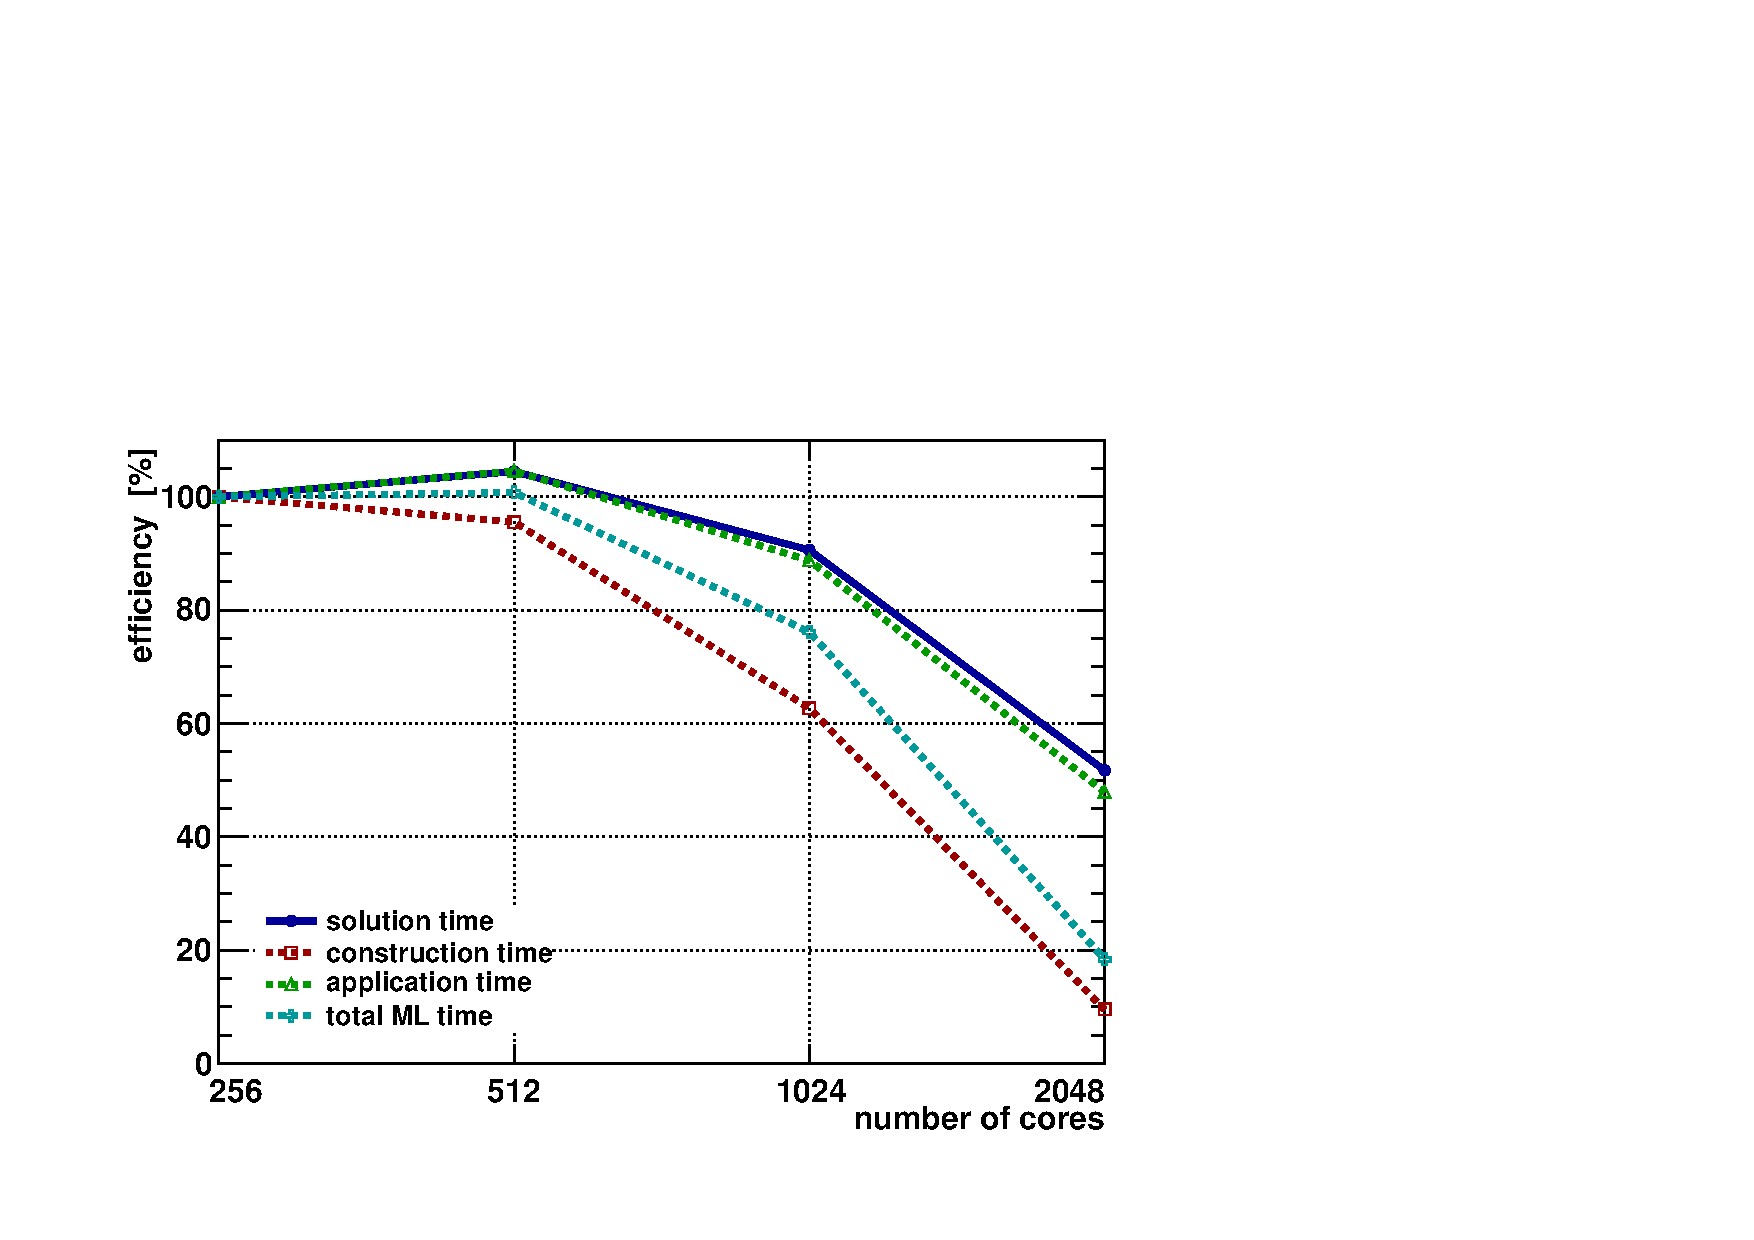
\includegraphics[width=0.45\textwidth]{figures/eff_512.pdf}
%  \caption{Efficiency for AMG on a tube embedded in a $512\times512\times512$
%  grid with constant extrapolation at the boundary \label{fig:speedup_512}}
%\end{center} 
%\end{figure}

Similar conclusions can be drawn for the parallel efficiency of our
solver on a $512^3$ grid with constant boundary treatment, see
Tab.~\ref{tbl:timings_solver_512} and Fig.~\ref{fig:speedup}.  Again the
construction phase of ML scales poorly for larger numbers of cores.

Notice that by applying the improvements discussed in
Section~\ref{sec:ml_var}, i.e., reusing (parts of) the preconditioner,
the time needed for the construction phase can be reduced significantly
or avoided altogether.  If the preconditioner has to be built just once
in an entire simulation the efficiency will get close to the 52\% that
we measured for the solution phase.  


Finally, in Tab.~\ref{tbl:timings_solver_1024} we report on timings
obtained for the tube imbedded in a $1024\times1024\times1024$ grid.  In
Figure~\ref{fig:speedup_1024} the corresponding efficiencies are listed.
For this large problem we observe good efficiencies.  The solver runs at
82\% efficiency with 2048 cores relative to the 512-cores performance.
The construction phase is still performing the worst with an efficiency
of \%73.  In this setup the problem size is still reasonably large when
employing 2048 cores.  This consolidates our understanding of the
influence of the problem size on the low performance of the aggregation
in ML.

\begin{figure}[htb] 
  \begin{center}
    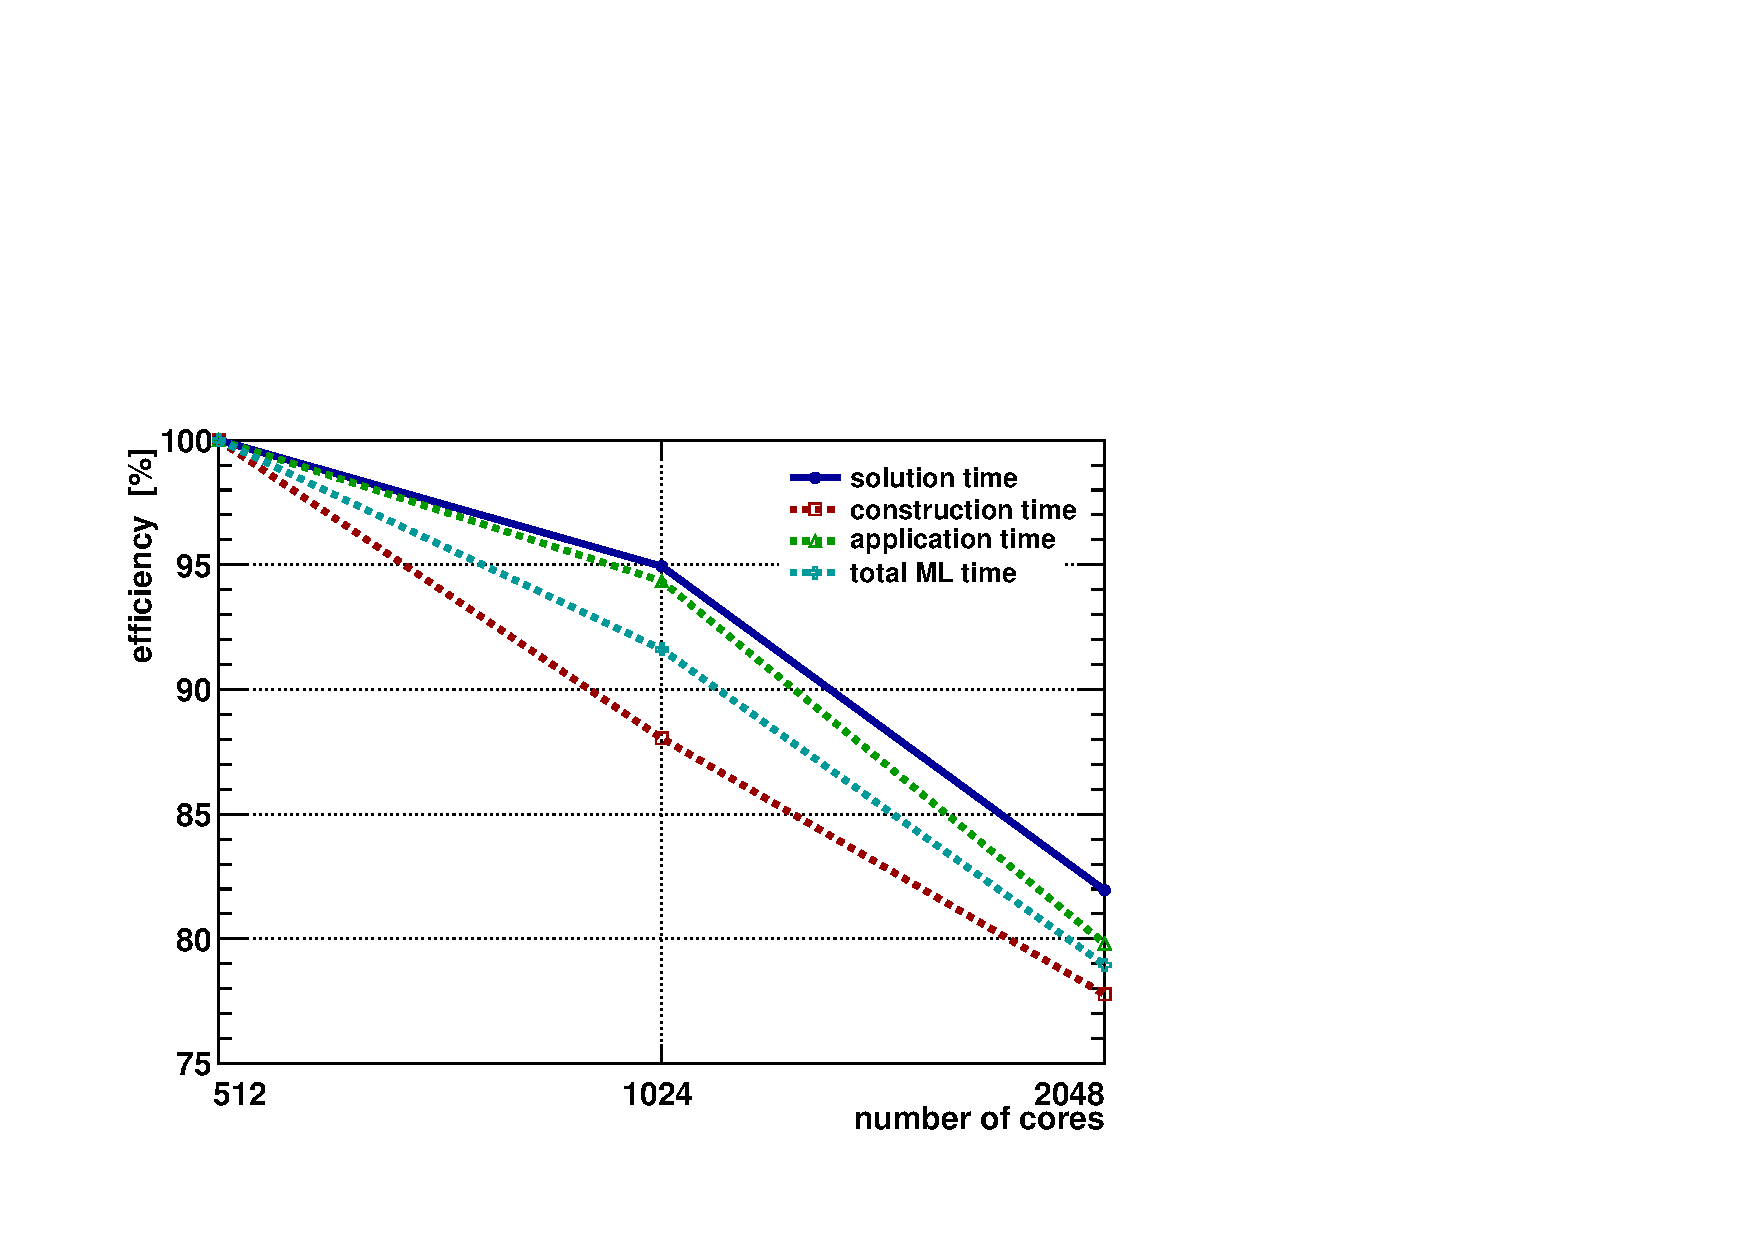
\includegraphics[width=0.5\textwidth]{figures/eff_1024_lin.pdf}
    \caption{Efficiency for AMG on a tube embedded in a
      $1024\times1024\times1024$ grid with linear extrapolation at the
      boundary \label{fig:speedup_1024}}
  \end{center} 
\end{figure}

\begin{table}[htb]
  \begin{center}
    \begin{tabular}{ccccc}
      \hline
      cores & solution [s] & construction [s] & application [s] & total ML [s] \\
%            & (s) & (s) & (s) & (s) \\
      \hline
      512  &  35.83 &  20.78 &  29.53 &  50.31  \\
      1024 &  18.87 &  11.80 &  15.65 &  27.46  \\
      2048 &  10.93 &  6.68 &  9.25 &  15.93   \\
      \hline
    \end{tabular}
    \caption{Timings for AMG on a tube embedded in a
      $1024\times1024\times1024$ grid with linear extrapolation at the
      boundary}
    \label{tbl:timings_solver_1024}
  \end{center}
\end{table}
%%

\subsection{Open-space vs.\ PEC Boundary Conditions} 
\label{sec:physrun}

In this section we compare the impact of two different boundary
conditions in the setting of a physical simulation consisting of an
electron source (1 MeV) followed by an iris with radius $r = 0.001$\,m.
The distance between the electron source and the beginning of the iris
is $0.006$\,m.  In order to compare the two boundary conditions we
inspected two properties of the particle bunch to be tracked
(integrated).  The first is the emittance (cf.~\cite[pp.154ff]{wied:07})
a measure of the phase-space volume i.e.\ of the beam quality measure.
Another property we observed is the root mean square (RMS) of the beam
size.  {\color{red}What the heck is this?}

In Figure~\ref{fig:vareps} we display emittance and RMS beam size for
the described simulation, once for open-space boundary conditions where
the potential approaches 0 at infinity and once for PEC boundary
conditions applied to the boundary of a cylinder with elliptical
base-area (as described in Section~\ref{sec:discr}).

%\begin{figure}[ht]
  %\begin{center}
    %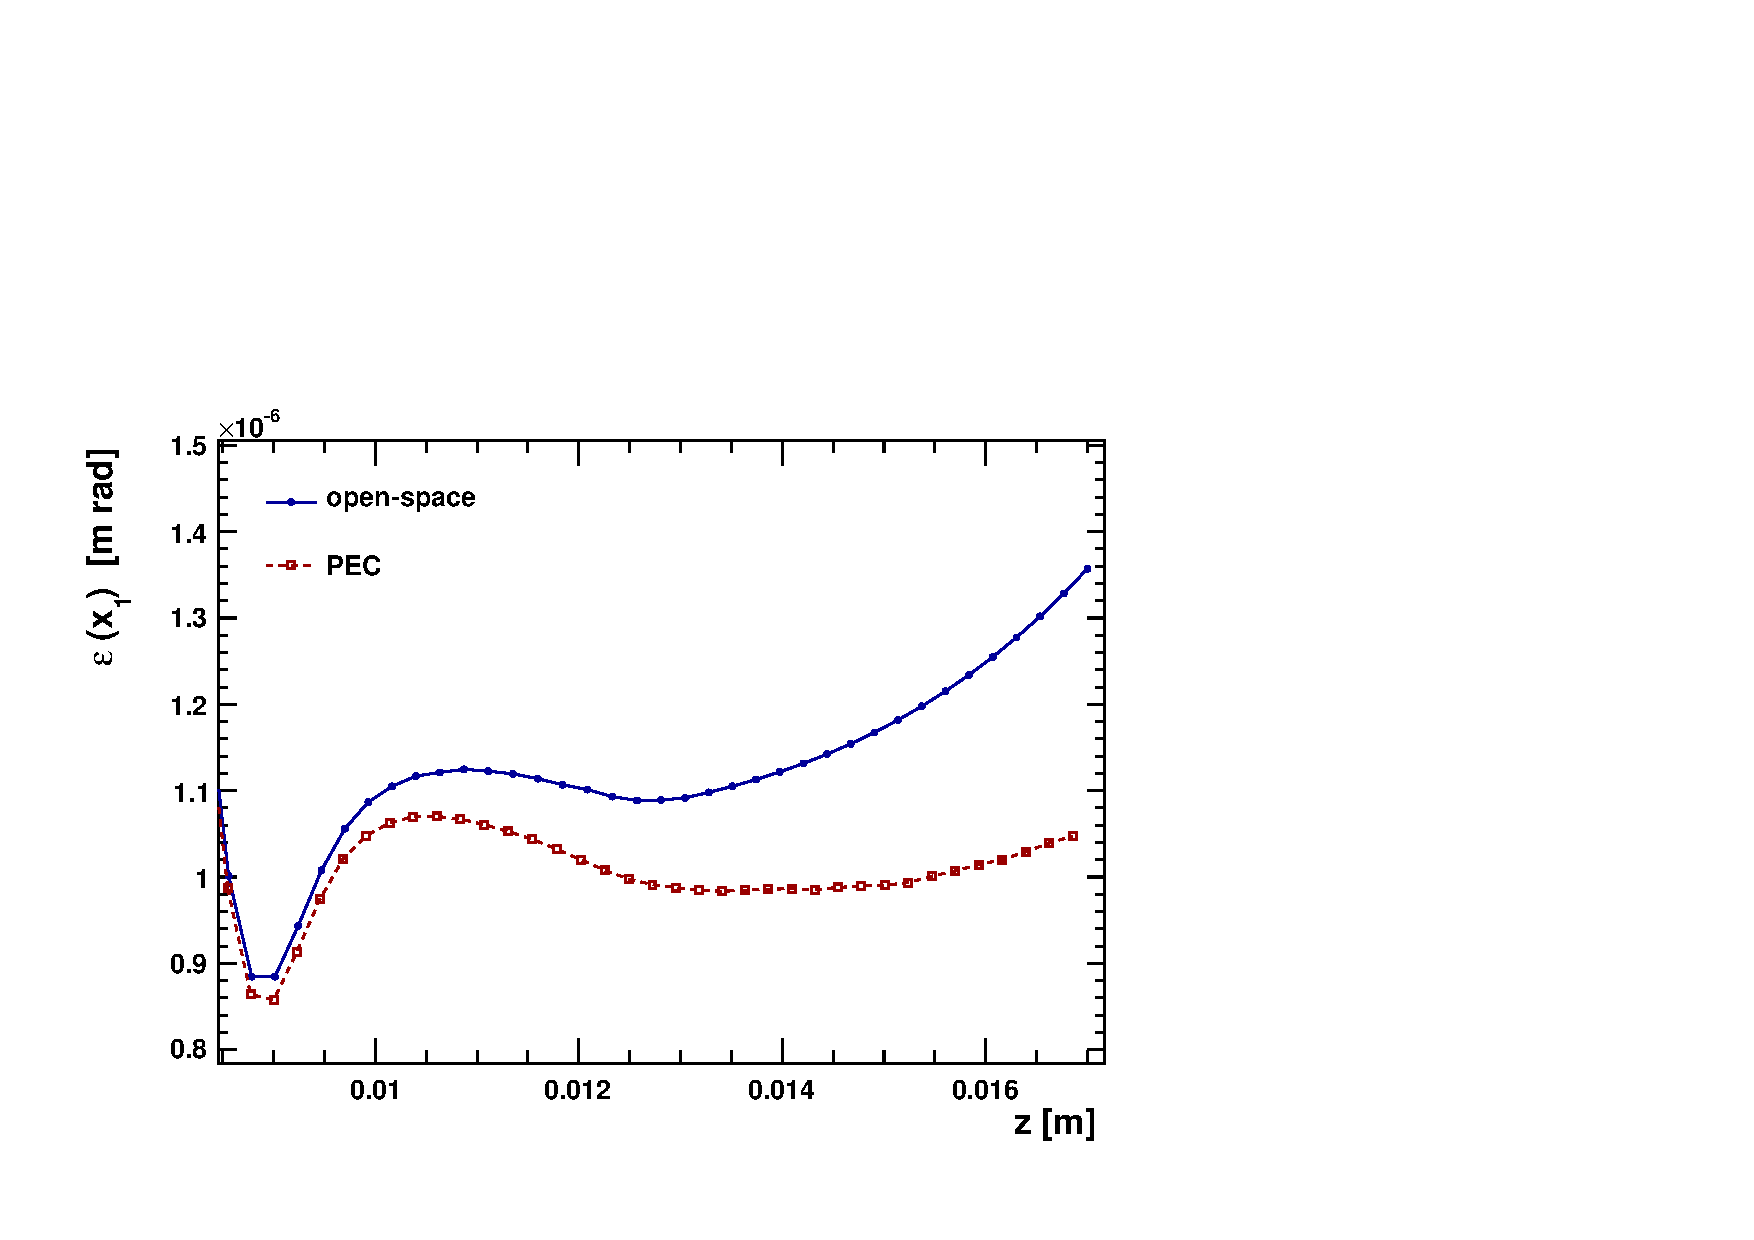
\includegraphics[width=0.45\textwidth]{figures/os_vs_pec_varepsilon_x.pdf}
    %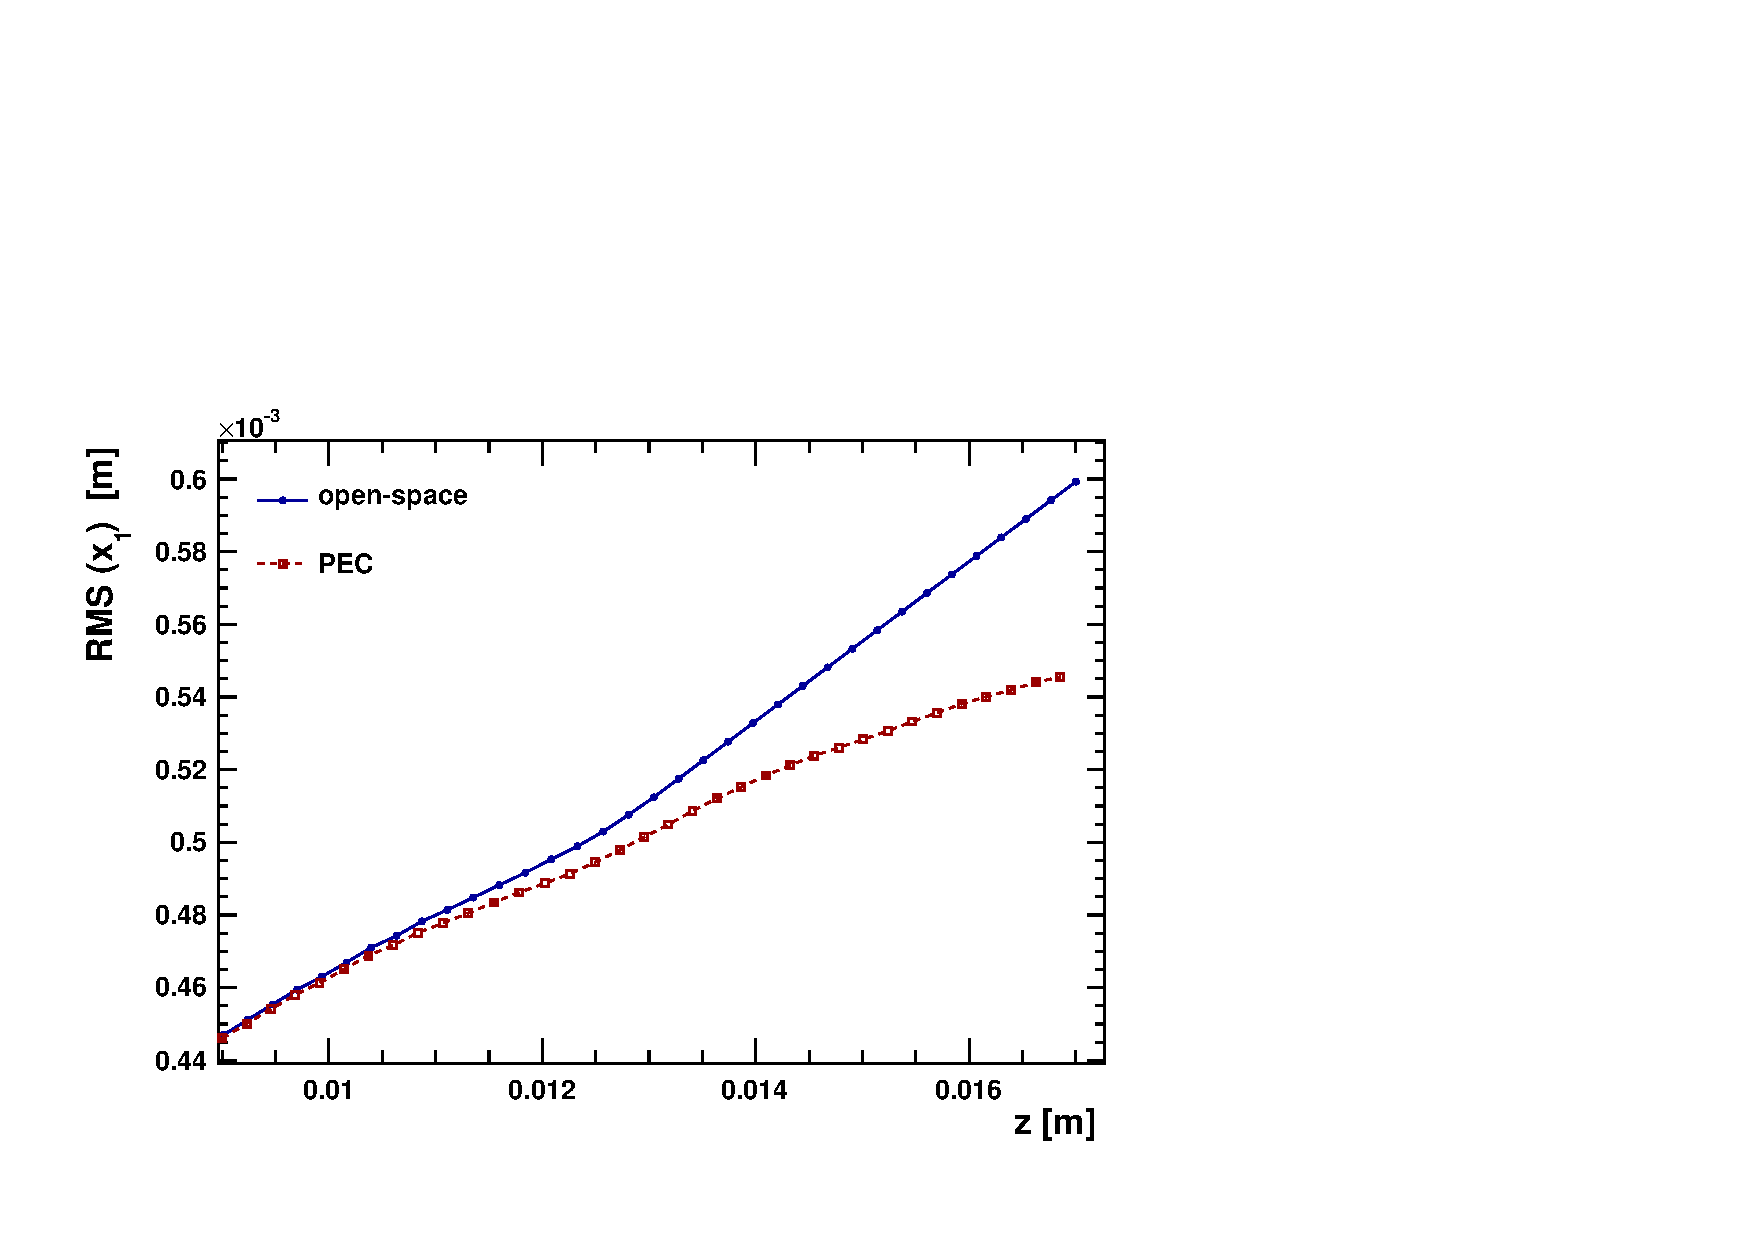
\includegraphics[width=0.45\textwidth]{figures/os_vs_pec_RMSX_x.pdf}
    %\caption{Comparison of emittance (left) and $\text{RMS}_{x_1}$ vs.\ position for open-space and PEC boundary conditions (region of interest
    %magnified). The computational domain $\Omega$ is a cylinder with $r=0.001$\,m  \label{fig:vareps}} 
  %\end{center} 
%\end{figure}

\begin{figure}[ht]
  \begin{center}
    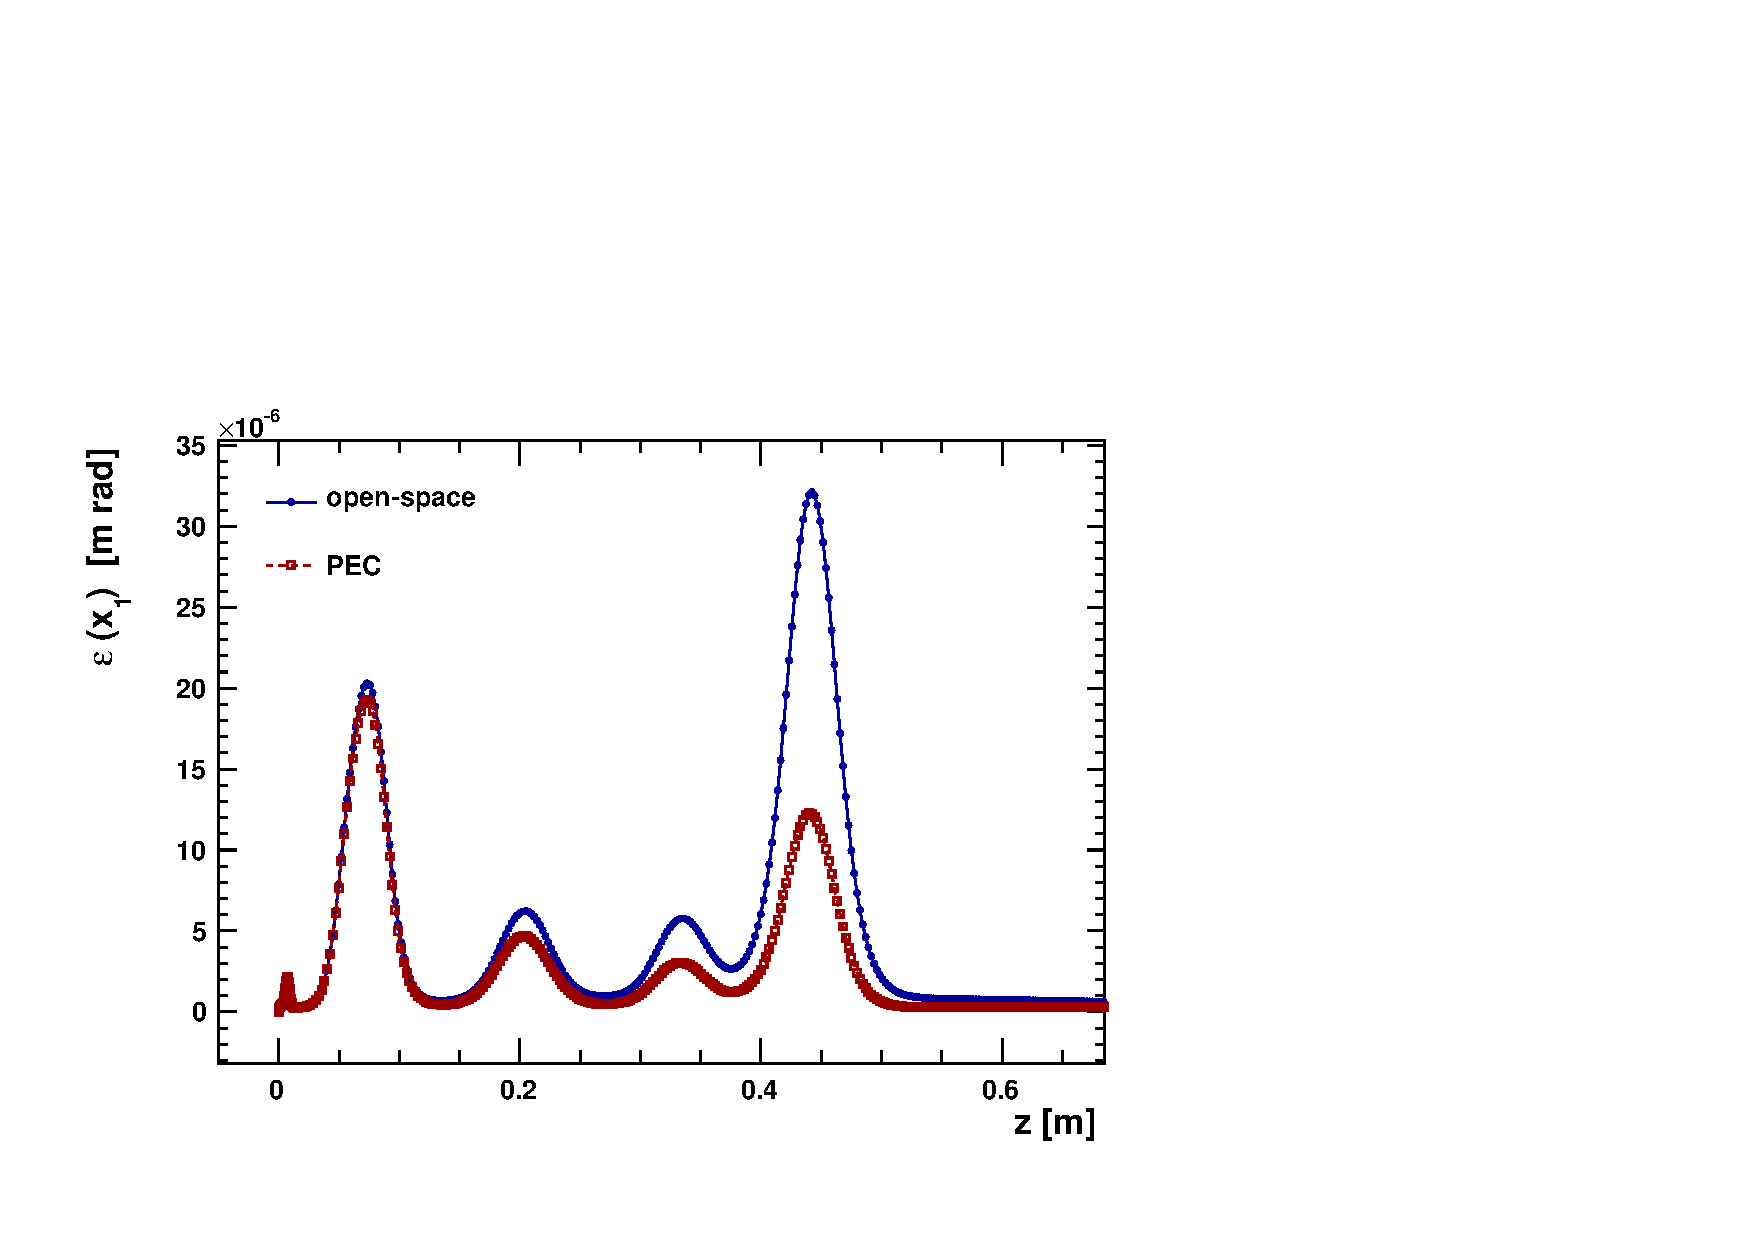
\includegraphics[width=0.5\textwidth]{figures/os_vs_pec_varepsilon_x_gun.pdf}
    \caption{Comparison of emittance vs.\ position for open-space and
      PEC boundary conditions (region of interest magnified). The
      computational domain $\Omega$ is a cylinder with
      $r=0.003$\,m \label{fig:vareps}.  {\color{red}Where are the RMS
        numbers?}}
  \end{center} 
\end{figure}

%TODO: compare paper PR ST AC E II 100703

The emittance shown in Figure~\ref{fig:vareps} is $30\%$ smaller (at
$z=0.016$\,m) for PEC boundary treatment compared to the open-space
approach, suggesting that space-charge forces are smaller when taking
into account ``realistic'' beam pipe boundaries.
% This results agree with physical prediction (intuition?) and numerical
% comparisons of electrostatic potentials.
This increase in accuracy justifies the necessity for an appropriately
accurate boundary treatment.

{\color{red}Explain why PEC is more accurate than open-space!}

%%% Local Variables: 
%%% mode: latex
%%% TeX-master: "paper"
%%% End:
